\subsubsection{Statistical Consistency}
To further validate our visual analysis, we can look at quantitative measures such as the means and standard deviations of \ce{SiO_2} concentrations across the folds and the overall dataset.

\begin{figure*}[htbp]
    \centering
    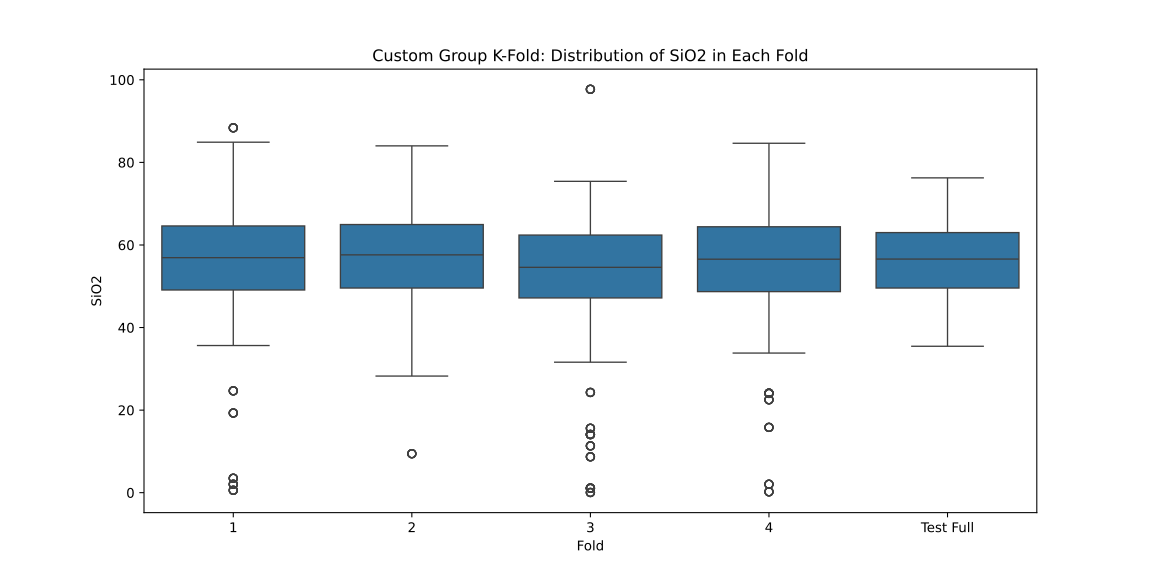
\includegraphics[width=\textwidth]{images/distribution_plot.png}
    \caption{Distribution of \ce{SiO_2} concentrations across cross-validation folds, training set, test set, and the entire dataset. The mean and standard deviation statistics for each partition are indicated figure.}
    \label{fig:siO2_distribution}
\end{figure*}

From Figure~\ref{fig:siO2_distribution}, it is evident that the means and standard deviations of \ce{SiO_2} concentrations for each fold are consistent with those of the overall dataset.

These metrics demonstrate that the means and standard deviations of \ce{SiO_2} concentrations for each fold and the combined training set are consistent with those of the overall dataset.
This quantitative consistency supports the visual evidence in Section~\ref{sec:visual_analysis} that each fold is a reliable representative of the entire dataset.
Furthermore, we can see that the standard deviation in the training sets is higher than the standard deviation in the test set, which is expected given the reassignment of extreme values to the training sets.

Maintaining balanced and representative distributions in each fold is essential for training robust models.
It ensures that the models are not biased towards any specific subset of the data, which is crucial for their generalization to unseen data.
The balanced distributions across folds enable the model to be trained on diverse subsets of data, leading to better generalization.
This approach reduces the risk of overfitting and ensures that the model performs well on new, unseen data.

By ensuring that each fold is representative of the overall dataset, these visualizations support the validity of our dataset partitioning strategy.
The consistency observed across folds further supports the claim that the data distribution method works as intended, providing confidence in the generalizability and reliability of our models.
